% !TEX TS-program = xeLaTeX
\documentclass[aspectratio=169,xcolor=x11names,compress]{ctexbeamer}
\usetheme{Darmstadt}
\useoutertheme[subsection=false,footline=authortitle]{miniframes}
\usefonttheme[onlymath]{serif}
\usepackage{setspace}
\usepackage{hyperref}
\usepackage{tikz}
\usepackage{graphicx}
\usepackage{booktabs}
\usepackage{amsmath}
\usepackage{listings}
\usepackage{xcolor}
\setstretch{1.2}
\CTEXoptions[today=old]

\input{beamer_template/beamer/format.tex}

\lstset{
 basicstyle=\ttfamily\footnotesize,
 keywordstyle=\color{blue},
 commentstyle=\color{green!50!black},
 stringstyle=\color{red!60!black},
 numbers=left,
 numberstyle=\tiny,
 breaklines=true,
 frame=single,
 columns=flexible,
 showspaces=false,
 showstringspaces=false,
}

\title{从象似性与组合性视角看《地书》图形语言与自然语言的异同}
\subtitle{——基于经典NLP与Transformer方法的对比分析}
\author{}
\date{\today}

\begin{document}

% ========== 标题页 ==========
\begin{frame}[plain]
\titlepage
\end{frame}

% ========== 目录 ==========
\begin{frame}{目录}
\tableofcontents
\end{frame}

% ========== 1. 研究背景与问题 ==========
\section{研究背景与问题}

\begin{frame}{研究背景：徐冰《地书》}
\textbf{《地书》（Earth Book）}——徐冰创作的一套完全由公共标识图形构成的叙事系统。

\vspace{0.5em}
\begin{columns}
\begin{column}{0.6\textwidth}
\begin{itemize}
    \item 使用图形符号而非文字进行叙事
    \item 与《天书》形成对偶：从不可读到人人可读
    \item 挑战"文字是语言唯一载体"的传统认知
    \item 核心语言学维度：\textbf{象似性（Iconicity）}与\textbf{组合性（Compositionality）}
\end{itemize}
\end{column}
\begin{column}{0.35\textwidth}
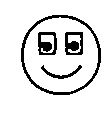
\includegraphics[width=0.9\textwidth]{examples/ex2_smile.jpg}
\centering\footnotesize 图形示例：seg\_003470 ``微笑''
\end{column}
\end{columns}

\vspace{0.5em}
\textbf{核心问题：}图形语言的象似性与组合性如何体现？与自然语言有何异同？
\end{frame}

\begin{frame}{研究问题（RQ）}
\begin{enumerate}
    \item \textbf{RQ1}：地书图形的象似性分布特征是什么？与自然语言词汇分布有何异同？
    \item \textbf{RQ2}：地书图形组合的组合性程度如何？是否表现出类似自然语言的层级组织？
    \item \textbf{RQ3}：经典NLP与Transformer方法在刻画两类语言异同方面各有何优势？
    \item \textbf{RQ4}：篇章关系分布反映了图形叙事的何种认知特征？
\end{enumerate}
\end{frame}

% ========== 2. 数据与方法 ==========
\section{数据与方法}

\begin{frame}{数据来源：四组材料}
\begin{columns}
\begin{column}{0.48\textwidth}
\textbf{材料0：标注系统 V1.0}
\begin{itemize}
    \item 纯前端（Vanilla JS）
    \item 12,078个原子图形（Atom）
    \item 22个标注任务配置
    \item 三级数据模型：Atom / Group / Annotation
\end{itemize}

\vspace{0.3em}
\textbf{材料1：图形标注数据}
\begin{itemize}
    \item 365个词标注文件
    \item 342个句标注文件
    \item 7,066条字面对应词
    \item 6,728条POS标注
    \item 5,332条形态特征标注
\end{itemize}
\end{column}
\begin{column}{0.48\textwidth}
\textbf{材料2：白话文本标注}
\begin{itemize}
    \item 192个标注文件
    \item 同一标注框架下的直接可比数据
\end{itemize}

\vspace{0.3em}
\textbf{材料3：对比语料库}
\begin{itemize}
    \item 四库全书（古典汉语）
    \item 世界名著（现代翻译）
    \item THUcNews（新闻语料）
    \item 小说（约1,145万行）
    \item WikiSentences30k\_16Lans
\end{itemize}
\end{column}
\end{columns}
\end{frame}

\begin{frame}[fragile]{数据预处理流程}
\textbf{JSON标注文件解析：}

\vspace{0.3em}
\begin{lstlisting}[language=Python]
def load_json_files(pattern):
    files = glob.glob(pattern)
    records = []
    for f in files:
        try:
            with open(f, 'r', encoding='utf-8') as fh:
                data = json.load(fh)
            if not data: continue
            records.append((os.path.basename(f), data))
        except (json.JSONDecodeError, UnicodeDecodeError):
            continue  # 跳过异常文件
    return records

def extract_annotations_by_target(records, task_name):
    result = defaultdict(list)
    for _, data in records:
        for ann in data.get('annotations', []):
            config = ann.get('annotation_config', {})
            if config.get('name') == task_name:
                target_id = ann.get('target_id', 'unknown')
                values = ann.get('values', [])
                result[target_id].extend(values)
    return dict(result)
\end{lstlisting}
\end{frame}

\begin{frame}{分析方法：两条技术路径}
\begin{columns}
\begin{column}{0.48\textwidth}
\textbf{经典NLP方法}
\begin{itemize}
    \item POS-like Category 频次分布统计
    \item 语义基元（Semantic Primitives）编码
    \item 类形态特征（Morphological）提取
    \item 篇章关系（Discourse Relations）分类
    \item TF-IDF 区分性词汇分析
    \begin{itemize}
        \item 中文正则分词：\texttt{re.findall(r'[\textbackslash u4e00-\textbackslash u9fff]\{2,\}', t)}
        \item \texttt{max\_features=200}, \texttt{min\_df=2}
    \end{itemize}
\end{itemize}
\end{column}
\begin{column}{0.48\textwidth}
\textbf{Transformer方法}
\begin{itemize}
    \item \texttt{bert-base-chinese}
    \begin{itemize}
        \item 12层Transformer编码器
        \item 隐藏层维度：768
        \item 参数量：约1.02亿
        \item 预训练任务：MLM + NSP
    \end{itemize}
    \item [CLS] token隐藏层输出作为句子级语义表示
    \item 余弦相似度计算语义一致性
    \item PCA降维可视化（$k=2$）
    \item 采样：两组各500条（计算资源限制）
\end{itemize}
\end{column}
\end{columns}
\end{frame}

\begin{frame}[fragile]{BERT嵌入提取代码}
\begin{lstlisting}[language=Python]
def get_bert_embeddings(texts, tokenizer, model, batch_size=32, max_length=64):
    embeddings = []
    model.eval()
    with torch.no_grad():
        for i in range(0, len(texts), batch_size):
            batch = texts[i:i+batch_size]
            inputs = tokenizer(batch, return_tensors='pt', 
                               padding=True, truncation=True, 
                               max_length=max_length)
            outputs = model(**inputs)
            batch_emb = outputs.last_hidden_state[:, 0, :].cpu().numpy()
            embeddings.append(batch_emb)
    return np.vstack(embeddings)
\end{lstlisting}

\vspace{0.3em}
\textbf{语义一致性指标：}
\[
S_{\text{intra}}^{(D)} = \frac{1}{N(N-1)} \sum_{i \neq j} \cos(\mathbf{e}_i^{(D)}, \mathbf{e}_j^{(D)}), \quad
S_{\text{cross}} = \frac{1}{NM} \sum_{i,j} \cos(\mathbf{e}_i^{(D)}, \mathbf{e}_j^{(B)})
\]
\end{frame}

% ========== 3. 结果 ==========
\section{结果与发现}

\begin{frame}{RQ1：POS分布——边界标记主导}
\begin{columns}
\begin{column}{0.55\textwidth}
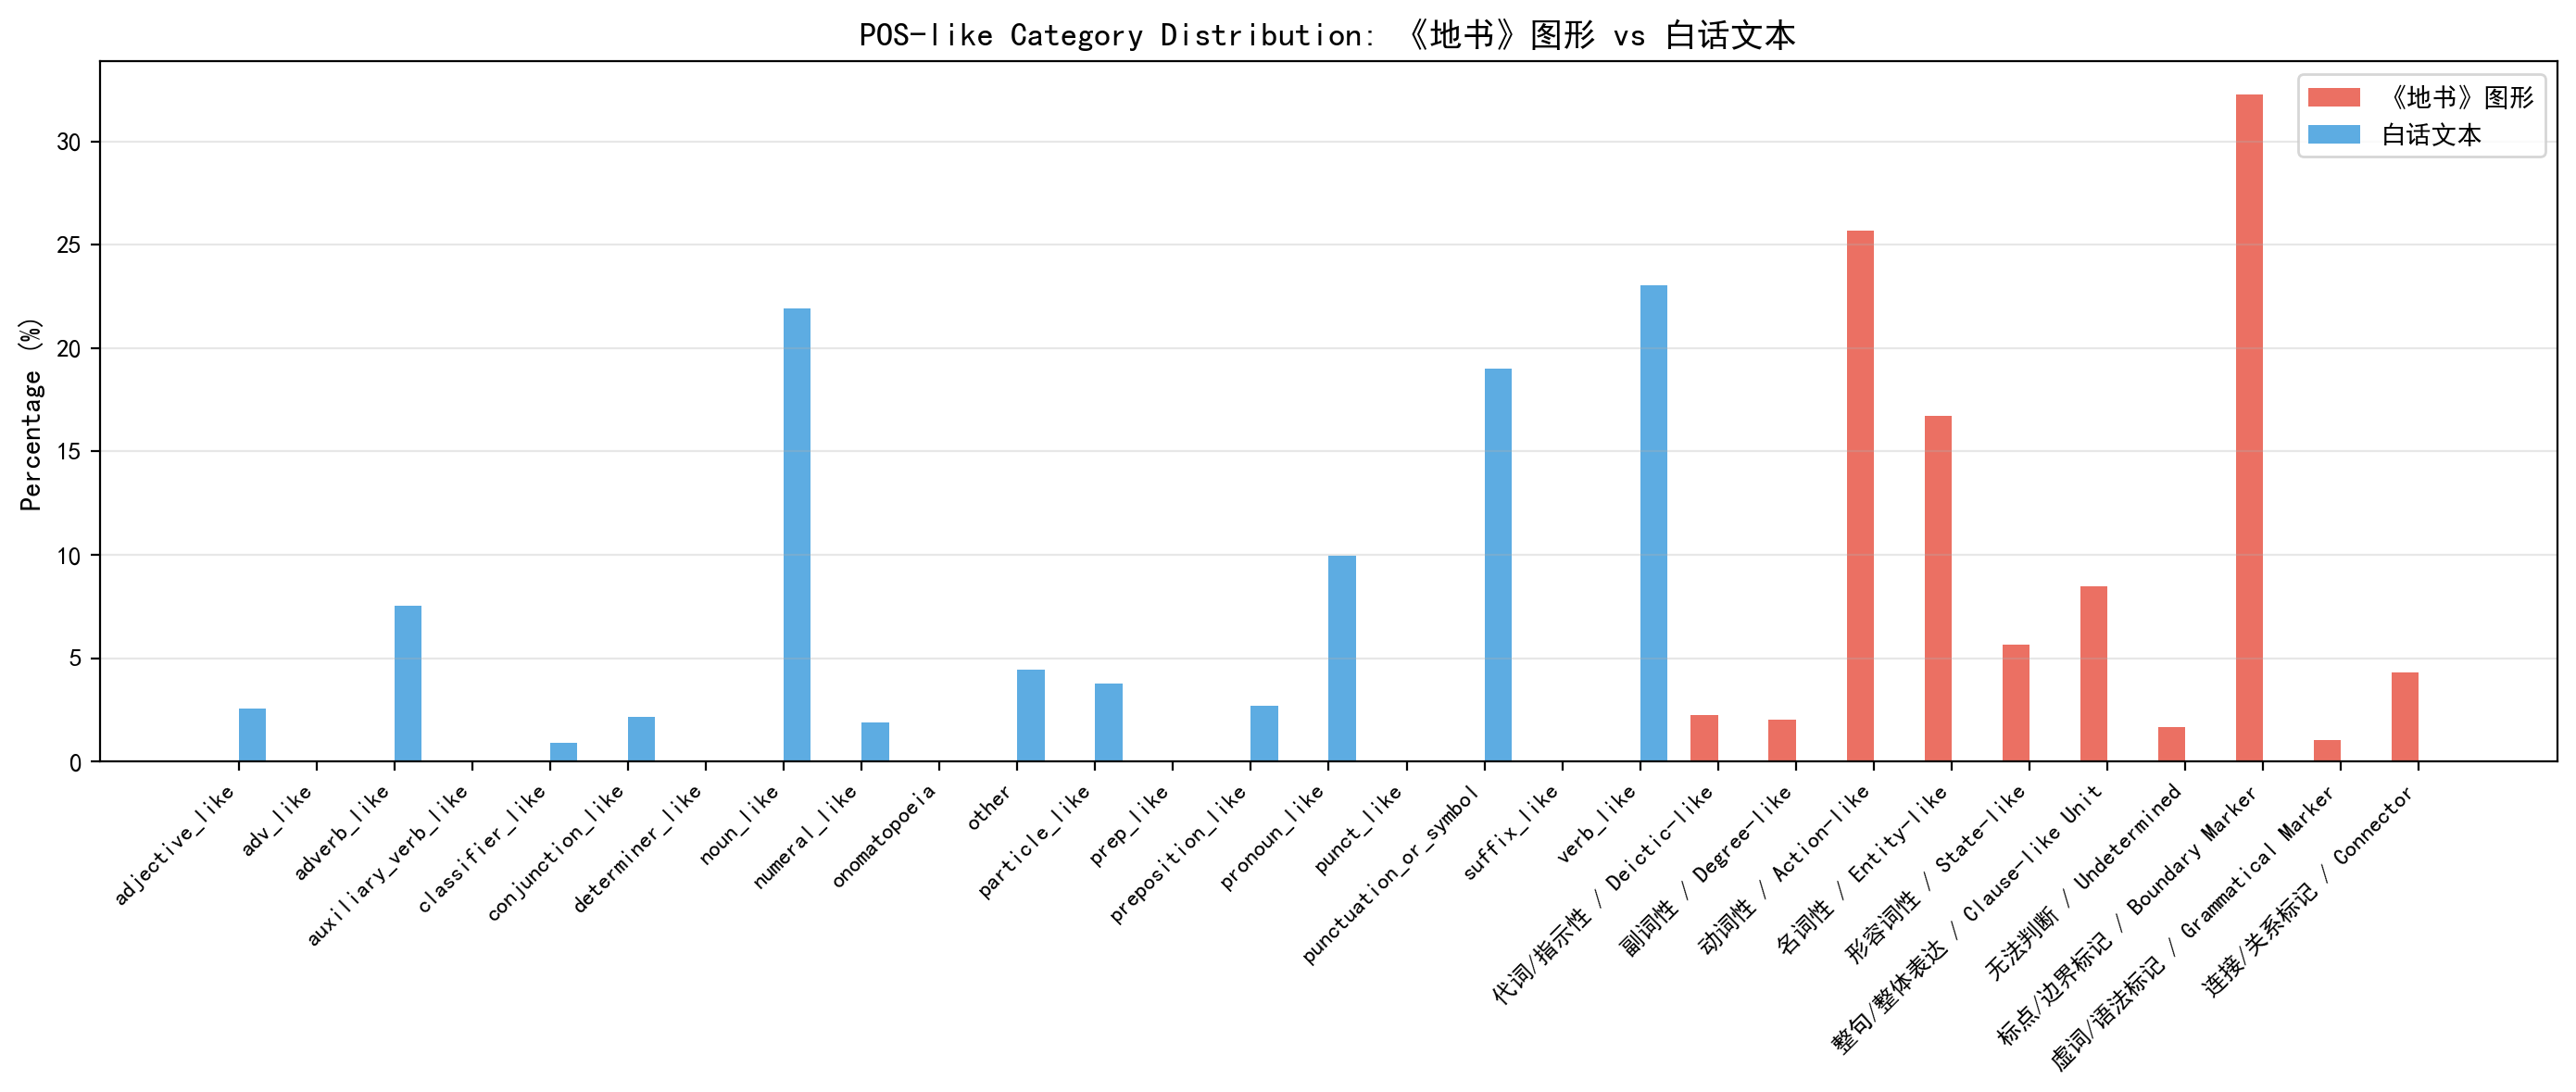
\includegraphics[width=\textwidth]{01_pos_distribution.png}
\end{column}
\begin{column}{0.42\textwidth}
\footnotesize
\begin{tabular}{lr}
\toprule
POS类别 & 占比 \\
\midrule
标点/边界标记 & \textbf{32.3\%} \\
动词性 / Action-like & 25.7\% \\
名词性 / Entity-like & 16.7\% \\
形容词性 / State-like & 7.5\% \\
整句/整体表达 & 8.5\% \\
连接/关系标记 & 4.3\% \\
虚词/语法标记 & 1.0\% \\
其他 & 4.0\% \\
\bottomrule
\end{tabular}

\vspace{0.3em}
\textbf{启示}：地书语法由\textbf{空间布局}编码，标点/边界标记占比远超自然语言（约19\%）。
\end{column}
\end{columns}
\end{frame}

\begin{frame}{RQ1：语义基元与形态特征}
\begin{columns}
\begin{column}{0.48\textwidth}
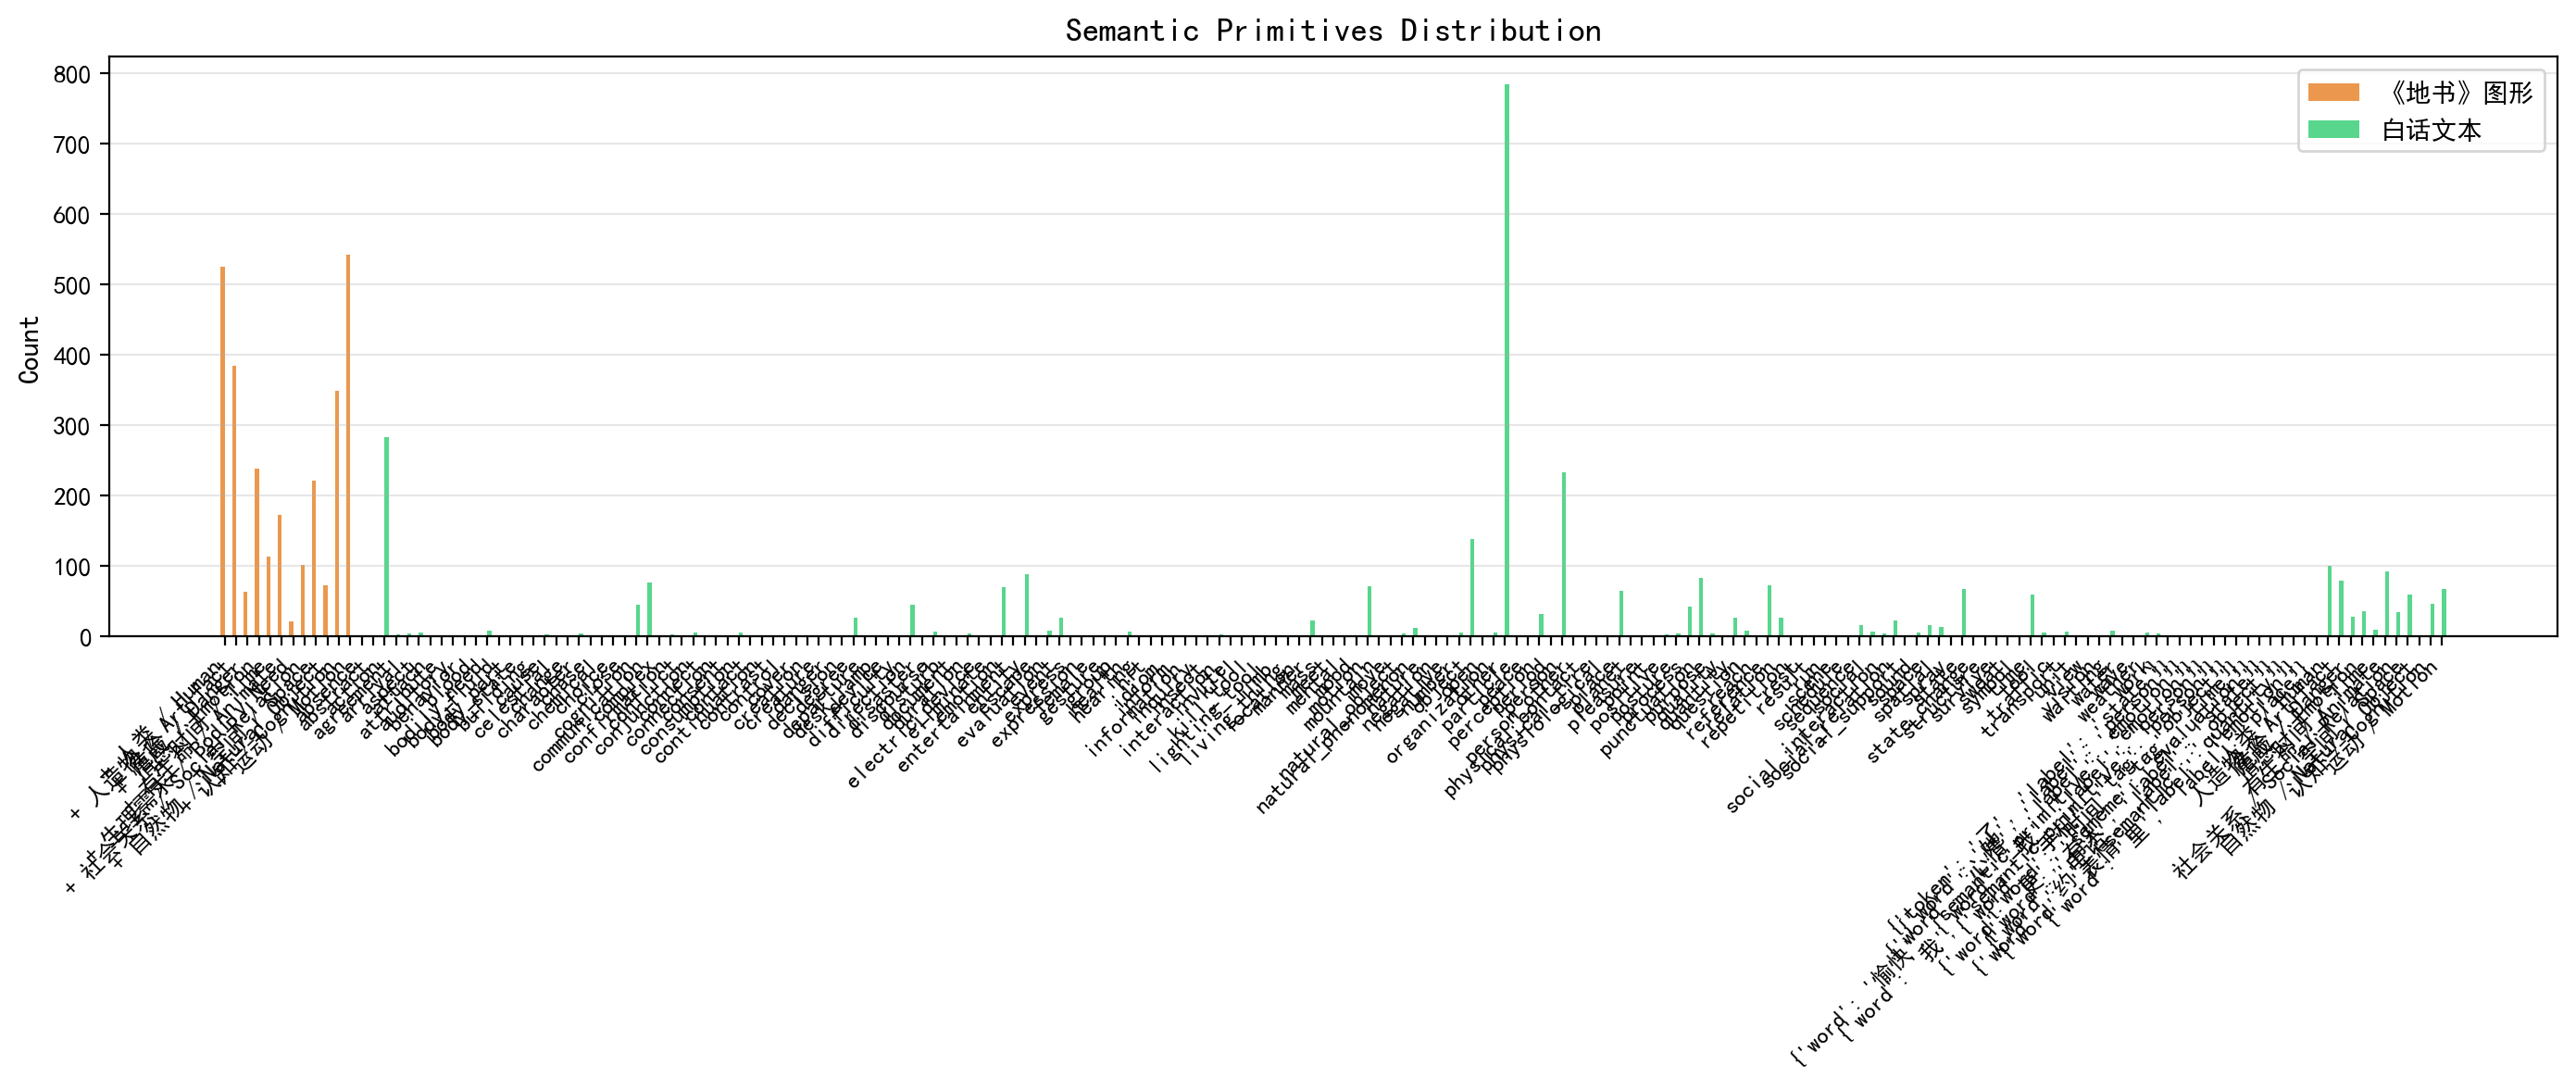
\includegraphics[width=\textwidth]{02_semantic_primitives.png}
\centering\footnotesize 语义基元分布

\vspace{0.3em}
\footnotesize
最频繁基元：\textbf{运动}、\textbf{情感}、\textbf{人类}、\textbf{有生命}
\end{column}
\begin{column}{0.48\textwidth}
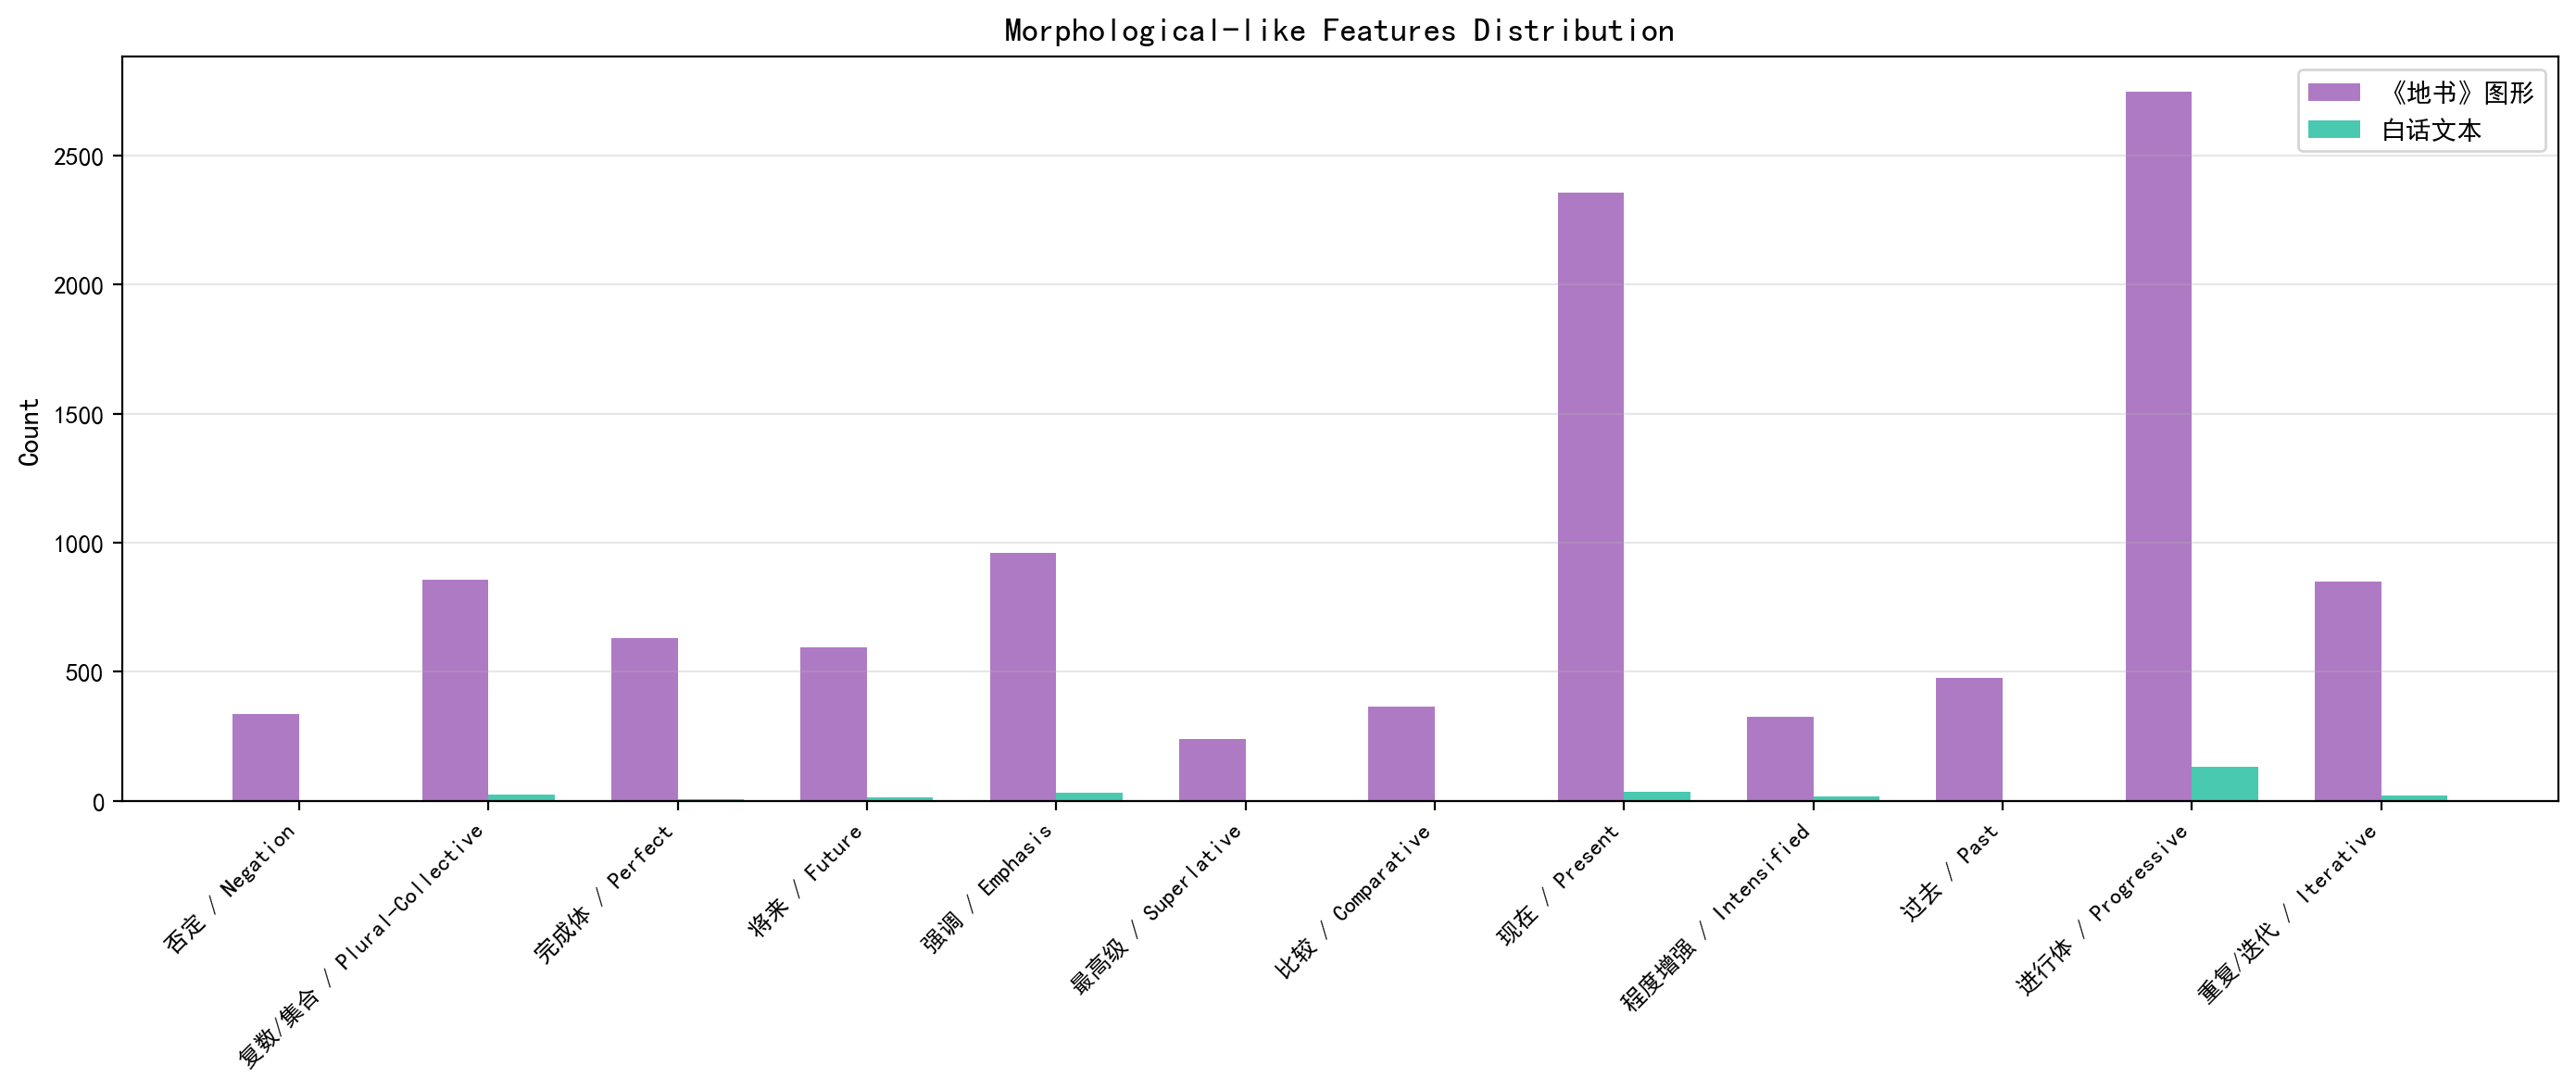
\includegraphics[width=\textwidth]{03_morphological_features.png}
\centering\footnotesize 形态特征分布

\vspace{0.3em}
\footnotesize
进行体：2,747次 \quad 现在时：2,356次

强调：960次 \quad 复数/集合：858次

白话仅281条形态标注
\end{column}
\end{columns}
\end{frame}

\begin{frame}{RQ1：自然语言参照对比}
\begin{columns}
\begin{column}{0.55\textwidth}
\footnotesize
\begin{tabular}{lcc}
\toprule
\textbf{指标} & \textbf{THUcNews} & \textbf{小说} \\
\midrule
总文档数 & 5,800 & 1,145万行 \\
平均句长（字） & 43.0 & 55--80 \\
标点密度 & 0.088 & 0.10--0.15 \\
\bottomrule
\end{tabular}

\vspace{0.5em}
自然语言功能词占比约15--25\%

\vspace{0.3em}
地书功能性元素（标点32.3\% + 连接4.3\% + 虚词1.0\%）合计约\textbf{37.6\%}
\end{column}
\begin{column}{0.42\textwidth}
\textbf{关键发现}：

\vspace{0.3em}
\footnotesize
若将标点/边界标记视为图形系统的``功能词等价物''，则地书的功能性元素比例实际上\textbf{高于}自然语言。

\vspace{0.3em}
差异在于编码模态：
\begin{itemize}
    \item 自然语言：时间线性
    \item 地书图形：空间二维
\end{itemize}
\end{column}
\end{columns}
\end{frame}

\begin{frame}{RQ2：组合性——"宽而浅"假说}
\begin{columns}
\begin{column}{0.55\textwidth}
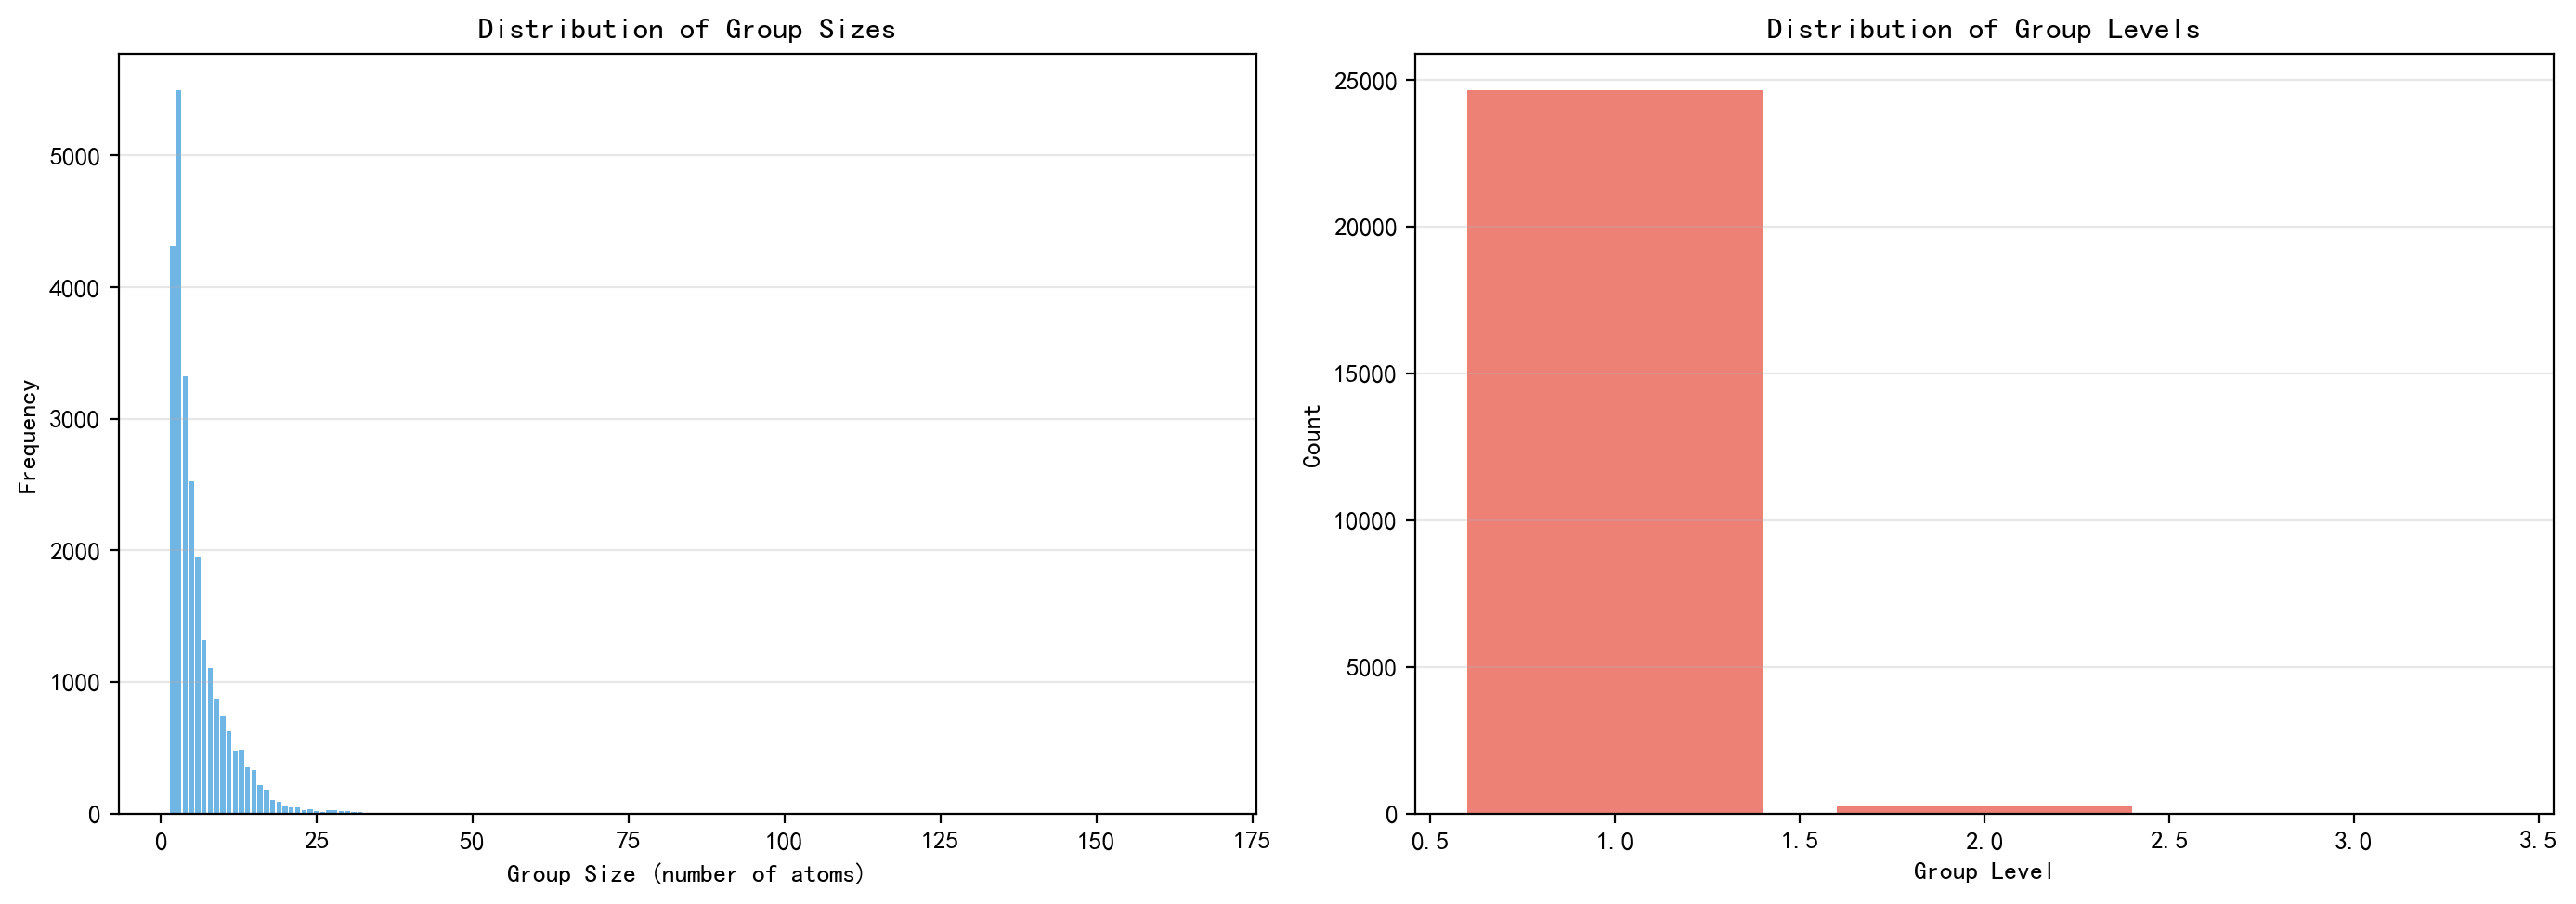
\includegraphics[width=\textwidth]{08_group_structure.png}
\end{column}
\begin{column}{0.42\textwidth}
\footnotesize
\begin{tabular}{lc}
\toprule
指标 & 数值 \\
\midrule
总分组数 & 24,930 \\
覆盖Atom数 & 8,317 / 12,078 \\
覆盖率 & 68.9\% \\
平均组大小 & \textbf{4.82}$\pm$4.06 \\
中位组大小 & 4 \\
Level 1占比 & \textbf{98.9\%} \\
Level 2+占比 & 1.1\%（285个） \\
\bottomrule
\end{tabular}

\vspace{0.3em}
\textbf{宽而浅组合性假设}：扁平并置为主，缺乏多层嵌套递归结构。
\end{column}
\end{columns}
\end{frame}

\begin{frame}{RQ3：TF-IDF语义焦点差异}
\begin{columns}
\begin{column}{0.55\textwidth}
\footnotesize
\textbf{地书图形Top 10区分词}：
\begin{tabular}{clc}
\toprule
Rank & 词汇 & Score \\
\midrule
1 & 逗号 & 0.0149 \\
2 & 双引号 & 0.0084 \\
3 & 冒号 & 0.0057 \\
4 & 圆点 & 0.0047 \\
5 & 感叹号 & 0.0041 \\
6 & 单引号 & 0.0041 \\
7 & 三辆车 & 0.0040 \\
8 & 省略号 & 0.0034 \\
9 & 括号 & 0.0034 \\
10 & 动作 & 0.0028 \\
\bottomrule
\end{tabular}
\end{column}
\begin{column}{0.42\textwidth}
\footnotesize
\textbf{白话文本Top 10区分词}：
\begin{tabular}{cl}
\toprule
Rank & 词汇 \\
\midrule
1 & 完成态 \\
2 & 蚊子 \\
3 & 男生说 \\
4 & 他们 \\
5 & 所有格 \\
6 & 调查 \\
7 & 我们 \\
8 & 助词 \\
9 & 女生说 \\
10 & 感到 \\
\bottomrule
\end{tabular}

\vspace{0.3em}
\textbf{启示}：图形释义依赖\textbf{空间关系}，文本释义依赖\textbf{语法与角色}。
\end{column}
\end{columns}
\end{frame}

\begin{frame}{RQ3：BERT语义嵌入分析}
\begin{columns}
\begin{column}{0.48\textwidth}
\footnotesize
\begin{tabular}{lccc}
\toprule
\textbf{Metric} & \textbf{Mean} & \textbf{Std} & \textbf{Median} \\
\midrule
地书组内 & 0.7697 & 0.1036 & 0.7819 \\
白话组内 & \textbf{0.7860} & 0.1044 & 0.7990 \\
跨组相似 & 0.7629 & 0.0948 & 0.7710 \\
\bottomrule
\end{tabular}

\vspace{0.5em}
\textbf{发现}：
\begin{itemize}
    \item 地书释义具有一致性（象似性约束）
    \item 白话更标准化（社区规范约束）
    \item 跨组差异约0.02--0.03
    \item BERT深层语义部分平滑了两组差异
\end{itemize}
\end{column}
\begin{column}{0.48\textwidth}
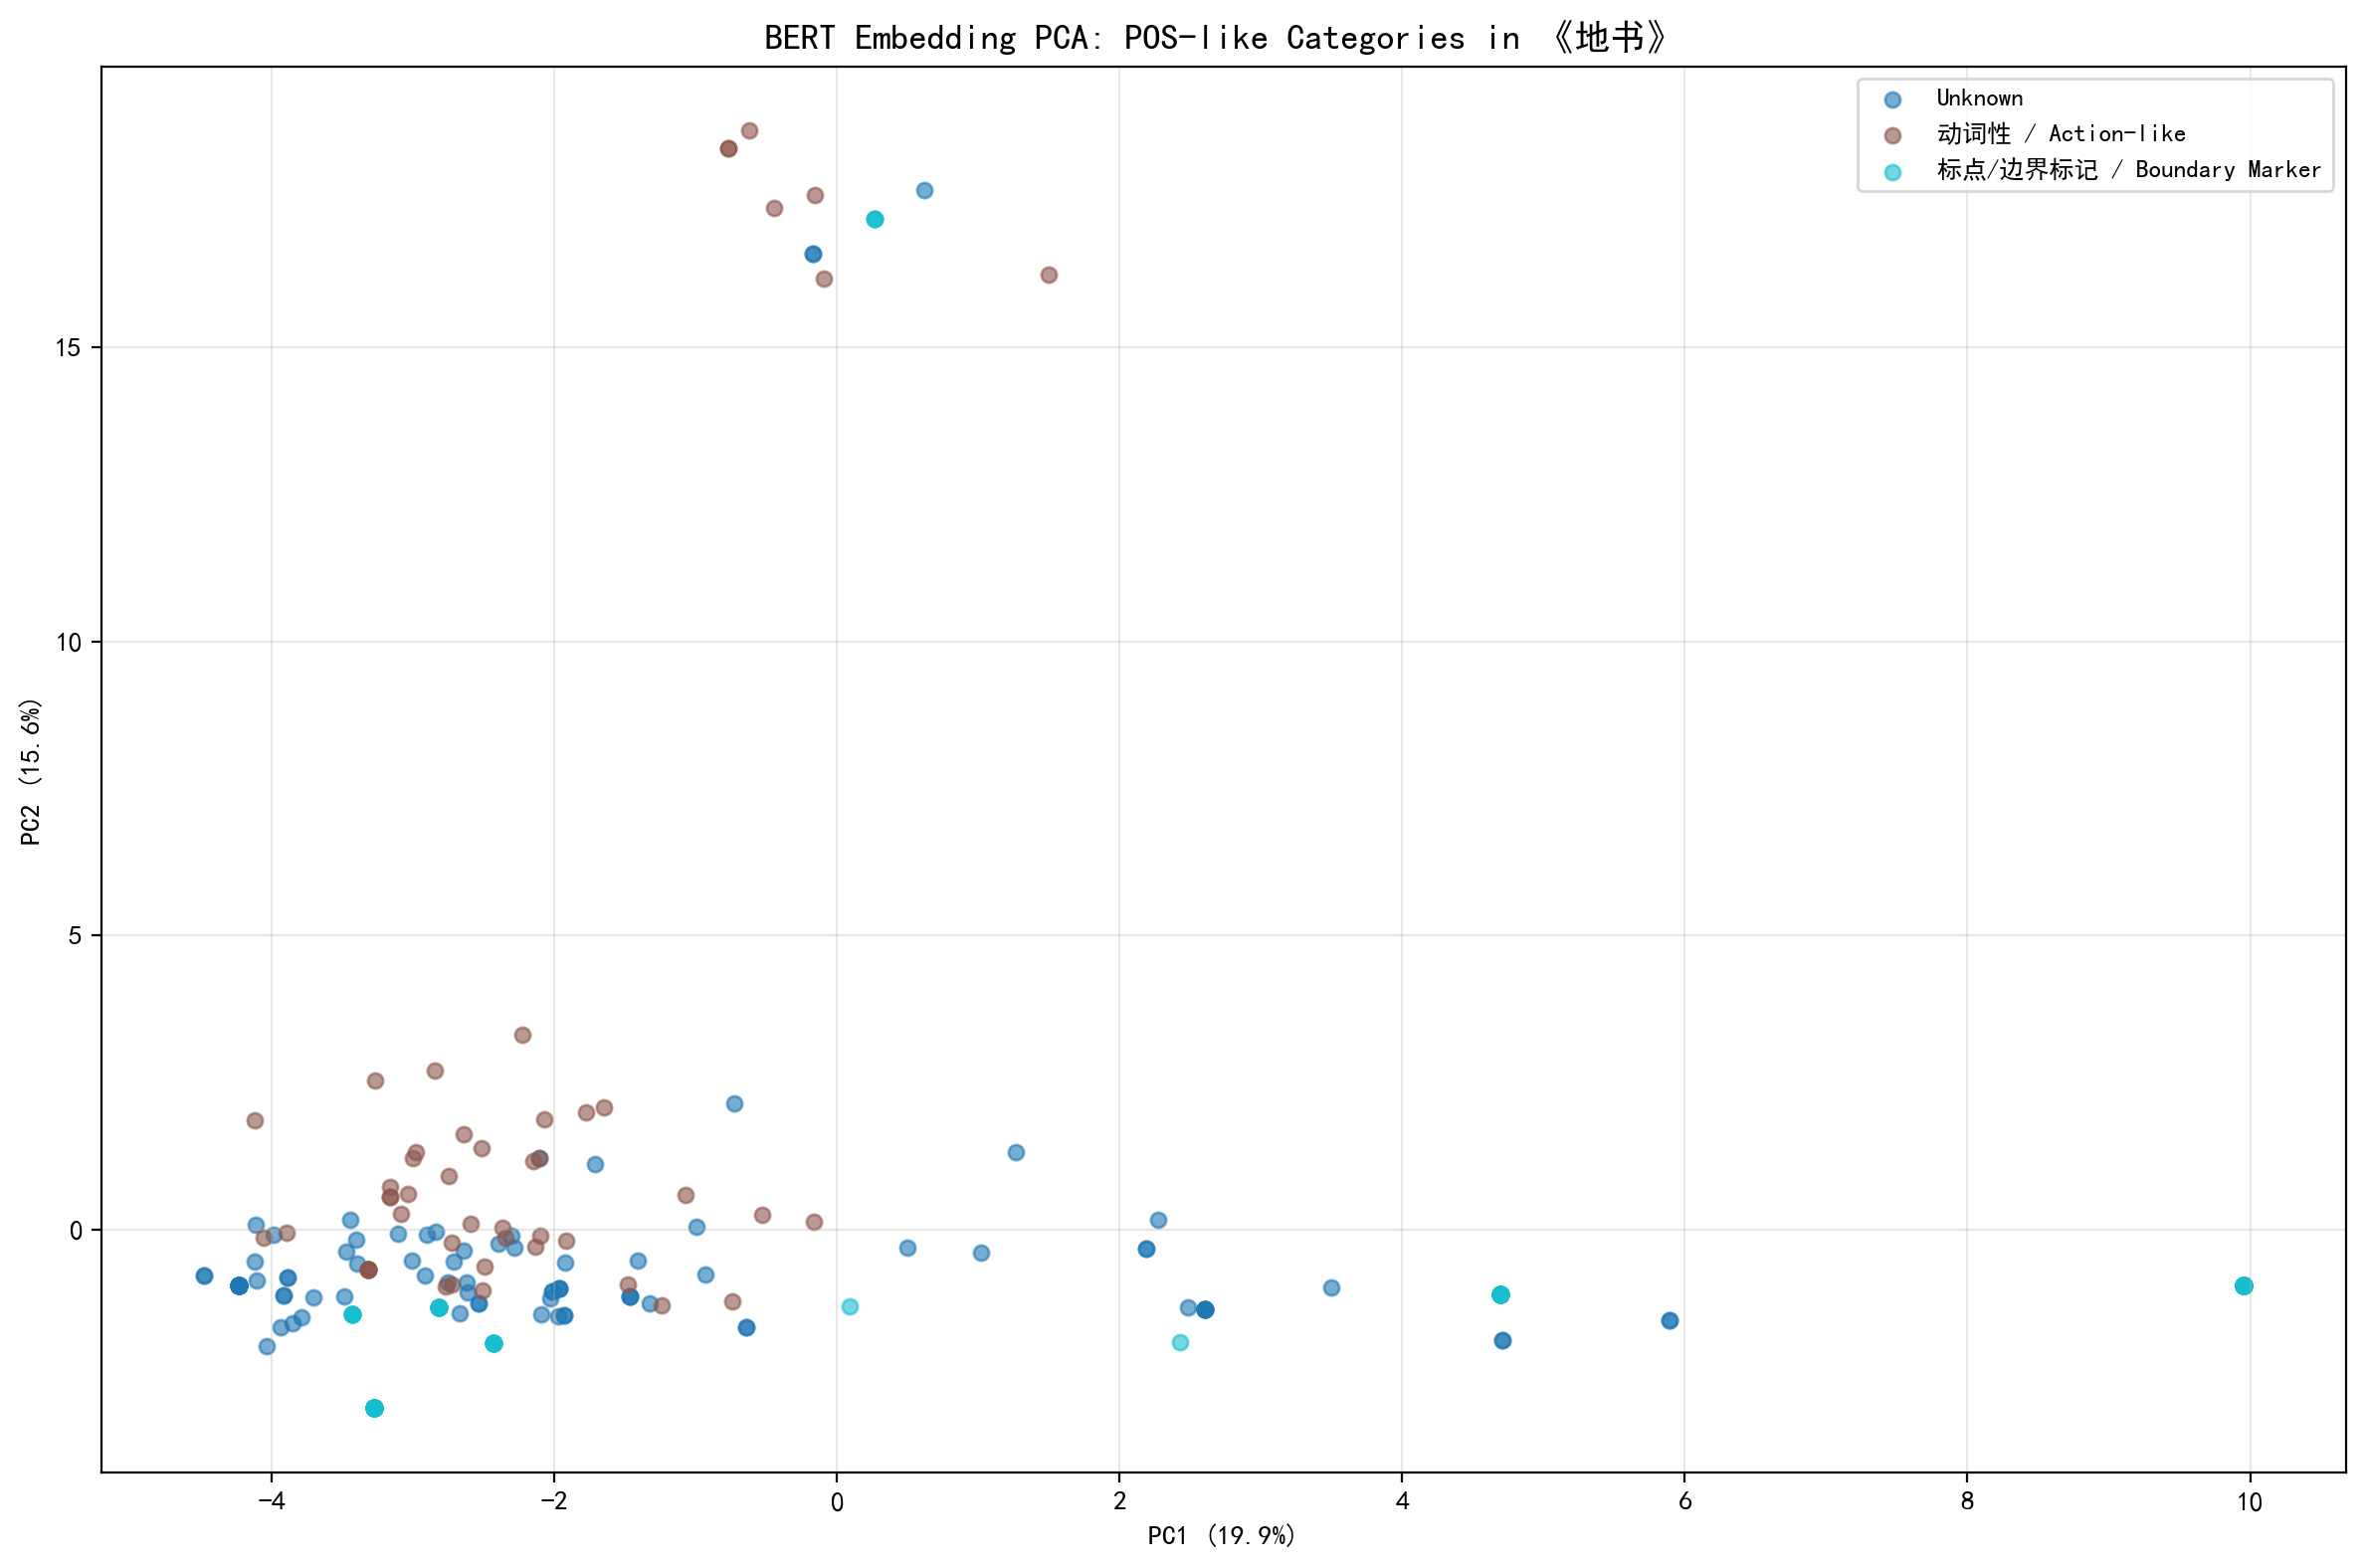
\includegraphics[width=\textwidth]{bert_pos_pca.png}
\centering\footnotesize PCA可视化：POS形成\textbf{连续语义梯度}
\end{column}
\end{columns}
\end{frame}

\begin{frame}{RQ3：BERT相似度分布}
\begin{columns}
\begin{column}{0.55\textwidth}
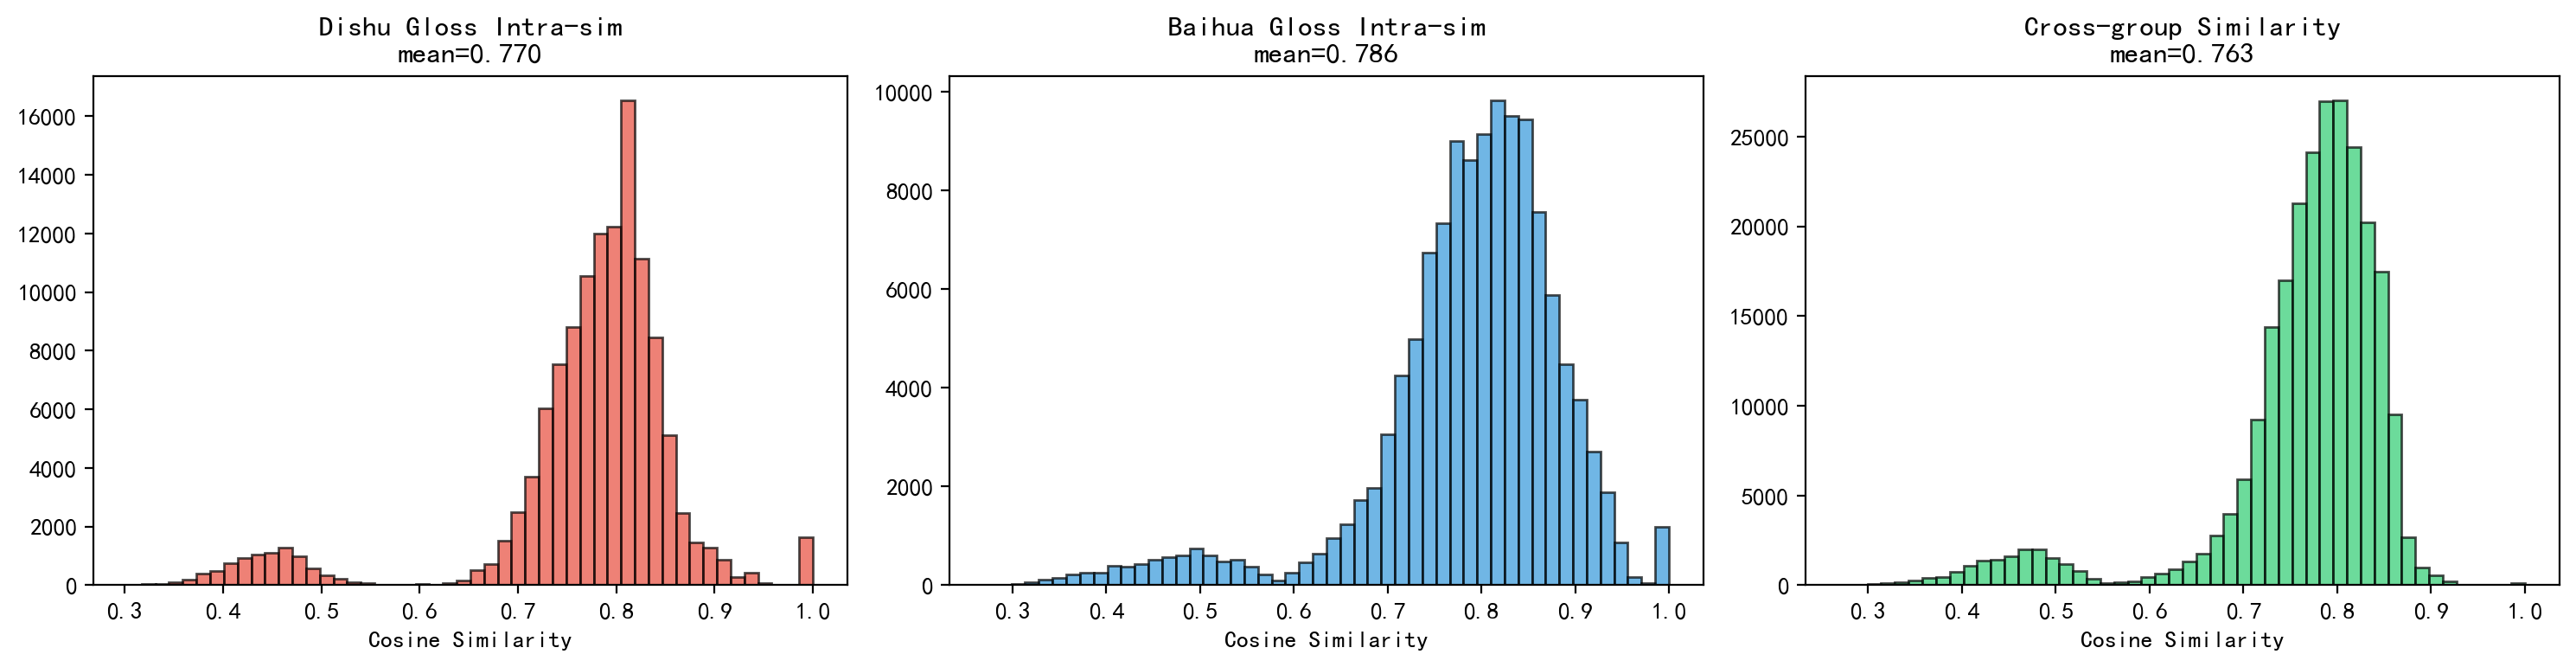
\includegraphics[width=\textwidth]{bert_similarity_distribution.png}
\end{column}
\begin{column}{0.42\textwidth}
\footnotesize
\textbf{三列分别为：}
\begin{itemize}
    \item 左：地书组内相似度分布
    \item 中：白话组内相似度分布
    \item 右：跨组相似度分布
\end{itemize}

\vspace{0.3em}
三组均值均在0.76--0.79之间，分布形态接近正态。

\vspace{0.3em}
\textbf{启示}：BERT训练数据中包含大量描述性文本，使得视觉描述与概念描述在向量空间中部分重叠。
\end{column}
\end{columns}
\end{frame}

\begin{frame}{RQ4：篇章关系——强时序叙事}
\begin{columns}
\begin{column}{0.55\textwidth}
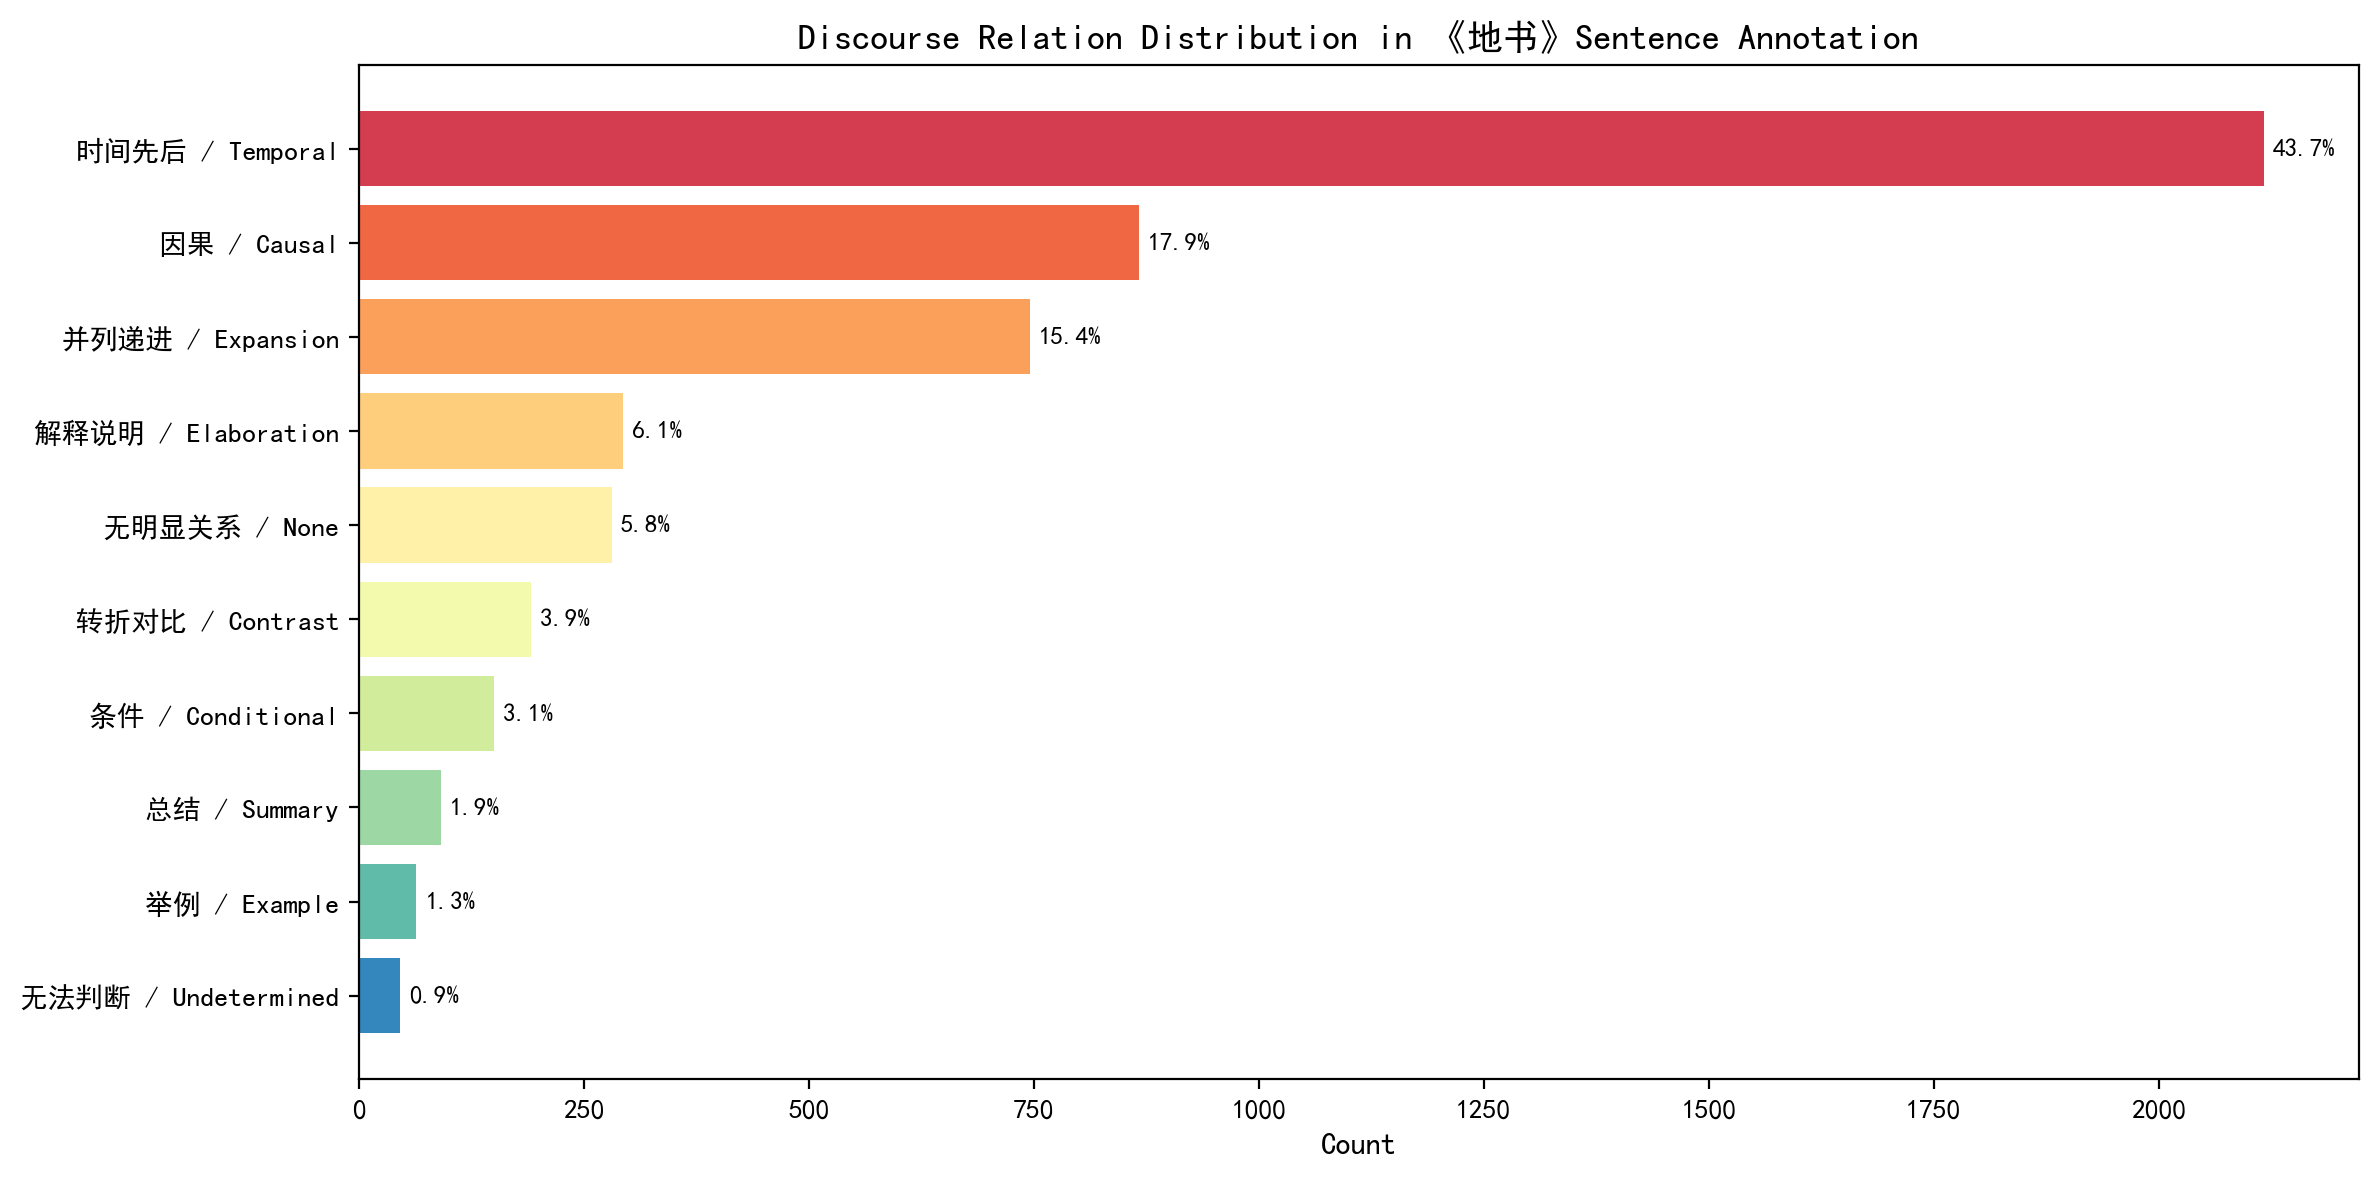
\includegraphics[width=\textwidth]{04_discourse_relation.png}
\end{column}
\begin{column}{0.42\textwidth}
\footnotesize
\begin{tabular}{lr}
\toprule
篇章关系 & 占比 \\
\midrule
时间先后 & \textbf{43.7\%} \\
因果 & 17.9\% \\
并列递进 & 15.4\% \\
转折 & 10.2\% \\
解释说明 & 4.6\% \\
条件 & 1.4\% \\
无明显关系 & 5.8\% \\
无法判断 & 0.9\% \\
\bottomrule
\end{tabular}

\vspace{0.3em}
\textbf{顺序象似性}（Givón, 1985）：事件物理先后顺序直接映射为图形空间先后顺序。
\end{column}
\end{columns}
\end{frame}

\begin{frame}{多维度发现汇总}
\footnotesize
\begin{columns}
\begin{column}{0.3\textwidth}
\textbf{象似性三维结构}
\begin{enumerate}
    \item 图形-概念象似性\\
    BERT组内0.770
    \item 序列-事件象似性\\
    时间先后43.7\%
    \item 组合-结构象似性\\
    组大小4.82
\end{enumerate}
\end{column}
\begin{column}{0.35\textwidth}
\textbf{空间拓扑标记}
\begin{itemize}
    \item 标点/边界标记32.3\%
    \item 功能等价物 $>$ 自然语言
    \item 二维空间编码替代时间线性编码
    \item 语法内嵌于视觉形式
\end{itemize}
\end{column}
\begin{column}{0.3\textwidth}
\textbf{方法互补性}
\begin{itemize}
    \item 经典NLP：宏观分布规律
    \item BERT：深层语义一致性
    \item TF-IDF：词汇焦点差异
    \item PCA：语义空间结构
\end{itemize}
\end{column}
\end{columns}
\end{frame}

% ========== 4. 结论 ==========
\section{结论与讨论}

\begin{frame}{主要结论}
\begin{enumerate}
    \item \textbf{象似性}：地书POS分布高度集中（边界标记32.3\%），象似性编码直接导致词性-视觉形态强绑定。BERT组内相似度0.770验证了语义约束强度。
    \item \textbf{组合性}：呈现``宽而浅"结构——平均组大小4.82$\pm$4.06，Level 1占98.9\%，深层嵌套仅1.1\%。与自然语言的递归句法形成对比。
    \item \textbf{语法编码}：空间拓扑标记（37.6\%）替代自然语言功能词（15--25\%）。语法关系由视觉布局和空间顺序编码，不存在形式与内容的分层。
    \item \textbf{叙事特征}：以动态事件为核心（运动/情感/人类基元主导），篇章关系以时序为主轴（43.7\%），缺乏条件/让步等复杂逻辑。
    \item \textbf{方法互补}：经典NLP揭示宏观结构规律（分布、TF-IDF、分组统计），BERT量化语义一致性（768维向量空间中的相似度）。
\end{enumerate}
\end{frame}

\begin{frame}{理论对话}
\begin{columns}
\begin{column}{0.48\textwidth}
\textbf{支持的理论}
\begin{itemize}
    \item Givón（1985）顺序象似性：时间先后43.7\%
    \item Jackendoff（2002）平行架构：语义驱动组合
    \item 认知语法组块化：组大小4.82 $\approx$ Miller 4组块
    \item 沈家煊名动包含：POS连续梯度
\end{itemize}
\end{column}
\begin{column}{0.48\textwidth}
\textbf{挑战的观点}
\begin{itemize}
    \item Chomsky（1957）递归性：地书缺乏深层递归
    \item 语言功能词必要性：地书无独立功能词
    \item 形式与内容分层：地书语法内嵌于视觉
\end{itemize}
\end{column}
\end{columns}

\vspace{0.5em}
\centering\footnotesize
\textbf{"宽而浅组合性假说"}：地书具有中等程度组合性——可线性组合形成内部结构单元，但缺乏递归嵌套机制。
\end{frame}

\begin{frame}{局限与未来工作}
\textbf{局限：}
\begin{itemize}
    \item 量表数据缺失：标注者未填写1--7分量表（iconicity、compositionality），无法直接对比主观评分
    \item BERT采样限制：两组各500条，可能存在长尾偏差
    \item 缺乏跨模态对比：未直接处理图形图像（仅分析标注文本）
    \item 标注一致性未评估：未计算Kappa系数
\end{itemize}

\vspace{0.5em}
\textbf{未来方向：}
\begin{itemize}
    \item 引入CLIP等多模态模型，直接对比图形图像与文本嵌入
    \item 更大规模标注一致性实验
    \item 与emoji、Blissymbolics等图形符号系统跨系统比较
    \item 基于LLM的地书自动翻译与生成验证
\end{itemize}
\end{frame}

\end{document}
